\documentclass{article}

\usepackage[top=2cm, bottom=2cm, left=1cm , right=1cm]{geometry}
\usepackage[utf8x]{inputenc}
\usepackage[T1]{fontenc}
\usepackage[francais]{babel}
\usepackage{amsmath, amssymb, amsthm}
\usepackage{mathrsfs}
\usepackage{enumitem}
\usepackage{graphicx}
\usepackage{ifthen}
\usepackage{fancyhdr}
\usepackage{pgf,tikz,pgfplots}
\usepackage{tkz-tab}
\usepackage{url}
\pgfplotsset{compat=1.15}
\usepackage{mathrsfs}
\usetikzlibrary{arrows}

% % % % % % % % % % % % % % % % % % % %
\newcounter{exo}
\newcounter{solution}
\newcommand{\exo}[1][NoTitle]{
        \setcounter{solution}{0}
  \refstepcounter{exo}
  \par\bigskip\noindent
  \textsc{\textbf{Exercice~\arabic{exo}}}
  \ifthenelse{\equal{#1}{NoTitle}}{}{\textbf{(#1)}}
  \quad\hrulefill
  \medskip\par
}
\newcommand{\solution}[1][NoTitle]{
  \refstepcounter{solution}
  \par\bigskip\noindent
  \textsc{\textbf{Solution question~\arabic{solution}}}
  \ifthenelse{\equal{#1}{NoTitle}}{}{\textbf{(#1)}}
  \quad\hrulefill
  \medskip\par
}
% % % % % % % % % % % % % % % % % % % %


\begin{document}

\exo{}
Soit $(C)$ la courbe définie par la représentation
\begin{align*}
\left\{%
\begin{array}{l}
x(t) = 3[t-\sin t]\\
y(t) = 3[1-\cos t]
\end{array}%
\right.
\end{align*}
\begin{enumerate}
        \item Étudier la partie de la courbe qui correspond à $t\in[\-pi;\pi]$.
                On notera $(\Gamma)$ cette partie de $(C)$.
        \item Démontrer que  $(C)$ se déduit de $(\Gamma)$ par des translations que l’on précisera.
\end{enumerate}
\solution{}
Pour étudier la courbe nous devons procéder en 3 étapes avant de la tracer~:
\begin{enumerate}
                \item Donner le domaine de définition et le domaine d'étude;
                \item donner le tableau de variations;
                \item compléter le tableau par l'étude des branches infinies s'il y en a.
\end{enumerate}
\section{Domaines de définition et d'étude: définition}
\subsection{Domaine de définition}
Le domaine de définition est l'ensemble des valeurs de $t$ telles que $x(t)$ et $y(t)$ existent.\\
\subsection{Domaine d'étude}
Le domaine d'étude est un sous domaine du domaine de définition.
Il est définit comme le plus petit domaine à étudier en prenant en compte
la périodicité et la parité de la fonction.
\subsubsection{Périodicité}
Si $D=\mathbb{R}$ et s'il existe $T$ tel que~:
\begin{align*}
\left\{%
\begin{array}{l}
        x(t+T) = x(t)\\
        y(t+T) = y(t)
\end{array}%
\right.
\end{align*}
alors la courbe a une période de $T$.
On peut donc l'étudier sur un intervalle de dimension $T$, $[\alpha;\alpha+T]$ avec $\alpha\in\mathbb{R}$.
On obtient toute la courbe en utilisant le fait que la courbe se répète à l'identique avec la période $T$.
\subsubsection{Parité}
Pour que la fonction ait une parité, il faut que son ensemble de définition soit
symétrique par rapport à $O$.
\begin{itemize}
                \item Si
\begin{align*}
\left\{%
\begin{array}{l}
        x(-t) = x(t)\\
        y(-t) = -y(t)
\end{array}%
\right.
\end{align*}
on étudie la courbe sur la partie positive de $D$, puis on fait la symétrie par
                rapport à $(Oy)$ pour obtenir la courbe sur la partie négative de $D$.
\begin{center}
        \begin{tikzpicture}
                \draw (0,-0.3) node[below,left]{$O$} ;
                \draw[->] (-1,0) -- (4,0);
                \draw (4,0) node[right] {$x$};
                \draw [->] (0,-4) -- (0,4);
                \draw (0,4) node[above] {$y$};
                \draw [dashed] (0,3) -- (2,3) node[right] {$y(t)$};
                \draw [dashed] (0,-3) -- (2,-3) node[below] {$y(-t)=-y(t)$};
                \draw (2,0.3) node[right] {$x(t)=x(-t)$};
                \draw [dashed] (2,3) -- (2,-3) ;
        \end{tikzpicture}
\end{center}
        \item Si
\begin{align*}
\left\{%
\begin{array}{l}
        x(-t) = -x(t)\\
        y(-t) = y(t)
\end{array}%
\right.
\end{align*}
on étudie la courbe sur la partie positive de $D$, puis on fait la symétrie par
                rapport à $(Oy)$ pour obtenir la courbe sur la partie négative de $D$.
\begin{center}
        \begin{tikzpicture}
                \draw (0,-0.3) node[below,left]{$O$} ;
                \draw[->] (-4,0) -- (4,0);
                \draw (4,0) node[right] {$x$};
                \draw [->] (0,-1) -- (0,4);
                \draw (0,4) node[above] {$y$};
                \draw [dashed] (2,3) -- (2,0) node[below] {$x(t)$};
                \draw [dashed] (-2,3) -- (-2,0) node[below] {$x(-t)=-x(t)$};
                \draw [dashed] (2,3) -- (0,3) node[above] {$y(t)=y(-t)$};
                \draw [dashed] (0,3) -- (-2,3);
        \end{tikzpicture}
\end{center}
        \item Si
\begin{align*}
\left\{%
\begin{array}{l}
        x(-t) = -x(t)\\
        y(-t) = -y(t)
\end{array}%
\right.
\end{align*}
on étudie la courbe sur la partie positive de $D$, puis on fait la symétrie par
                rapport à $O$ pour obtenir la courbe sur la partie négative de $D$.
\begin{center}
        \begin{tikzpicture}
                \draw (0,-0.3) node[below,left]{$O$} ;
                \draw[->] (-4,0) -- (4,0);
                \draw (4,0) node[right] {$x$};
                \draw [->] (0,-4) -- (0,4);
                \draw (0,4) node[above] {$y$};
                \draw [dashed] (2,3) -- (2,0) node[below] {$x(t)$};
                \draw [dashed] (2,3) -- (0,3) node[left] {$y(t)$};
                \draw [dashed] (-2,-3) -- (-2,0) node[above] {$x(-t)=-x(t)$};
                \draw [dashed] (-2,-3) -- (0,-3) node[right] {$y(-t)=-y(t)$};
        \end{tikzpicture}
\end{center}
\end{itemize}
\section{Domaines de définition et d'étude: application}
\subsection{Domaine de définition}
Dans le cas qui nous intéresse, $x(t) = 3[t-\sin t]$ et $y(t) = 3[1-\cos t]$ sont définies
quel que soit $t$.
Donc $D=\mathbb{R}$.
\subsection{Domaine d'étude}
\subsubsection{Périodicité}
Les fonctions $x(t)$ et $y(t)$ ne sont pas périodiques.
Donc la courbe n'a pas de périodicité.
\subsubsection{Parité}
On calcule $x(-t)$ et $y(-t)$~:
\begin{align*}
\left\{%
\begin{array}{l}
        x(-t) = 3[-t-\sin -t] = 3[-t+\sin t]=-x(t)\\
        y(-t) = 3[1-\cos -t] = 3[1-\cos t]=y(t)
\end{array}%
\right.
\end{align*}
On nous demande de travailler sur l'intervalle $[-\pi;\pi]$.
Dans ce cas, on peut réduire l'intervalle d'étude à la partie positive de $[-\pi;\pi]$, c'est-à-dire
$[0;\pi]$.
On construira la courbe sur $[-\pi;\pi]$ en faisant une symétrie par rapport à $(Oy)$.
\section{Tableau de variations}
\subsection{Variations}
On se place sur l'intervalle d'étude $I=[0;\pi]$.\\
On détermine les expressions suivantes:
\begin{align*}
        x'(t) = 3[1-\cos t]\\
        y'(t) = 3\sin t
\end{align*}
Comme $-1\le\cos t\le+1$, $x'(t)$ est toujours positive ou nulle.\\
Sur $[0;\pi]$, $\sin t\ge 0$ donc $y'(t)\ge 0$.\\
De plus,
\begin{align*}
        x (0) & = 3[0-\sin 0] = 0 & x (\pi) & = 3[\pi - \sin \pi] = 3\pi\\
        y (0) & = 3[1-\cos 0] = 0 & y (\pi) & = 3[1   - \cos \pi] = 6\\
        x'(0) & = 0               & x'(\pi) & = 6                    \\
        y'(0) & = 0               & y'(\pi) & = 0                    \\
\end{align*}
On a donc le tableau de variations suivant~:\\
\begin{tikzpicture}
        \tkzTabInit{$t$ / 1 , $x'(t)$ / 1, $x(t)$ / 1, $y'(t)$ / 1, $y(t)$ / 1}{$0$, $+\pi$}
        \tkzTabLine{0,+,6}
        \tkzTabVar{-/ $0$ , +/ $3\pi$}
        \tkzTabLine{0,+,0}
        \tkzTabVar{-/ $0$ , +/ $6$}
\end{tikzpicture}
\subsection{Tangentes}
On détermine les tangentes en $0$ et en $\pi$.
On cherche donc en ces points le premier vecteur dérivé non nul.\\
En $t=0$~:
\begin{align*}
        \vec{F}'(0)&=\left|\begin{array}{l}
                x'(0)\\y'(0)
        \end{array}\right.
        =          \left|\begin{array}{l}
                0\\0
        \end{array}\right.\\
        \vec{F}"(0)&=\left|\begin{array}{l}
                3\sin 0\\3\cos 0
        \end{array}\right.
        =          \left|\begin{array}{l}
                0\\3
        \end{array}\right.
\end{align*}
$\vec{F}"$ est donc le premier vecteur dérivé non nul en $0$, il dirigera donc la tangente en $0$.\\
En $t=\pi$~:
\begin{align*}
        \vec{F}'(\pi)&=\left|\begin{array}{l}
                x'(\pi)\\y'(\pi)
        \end{array}\right.
        =          \left|\begin{array}{l}
                6\\0
        \end{array}\right.\\
\end{align*}
$\vec{F}'$ est donc le premier vecteur dérivé non nul en $\pi$, il dirigera donc la tangente en $\pi$.
\section{Branches infinies}
Il n'y a ni borne infinie, ni valeur interdite, donc pas de branche infinie à étudier.
\section{Tracé de la courbe $(\Gamma)$}
On place les tangentes, les points pour lesquels on connaît les valeurs\footnote{ainsi
que quelques points pour lesquels on peut facilement calculer $x(t)$ et $y(t)$ si possible}.
On n'oublie pas de faire la symétrie de la courbe par rapport à $(Oy)$.\\
%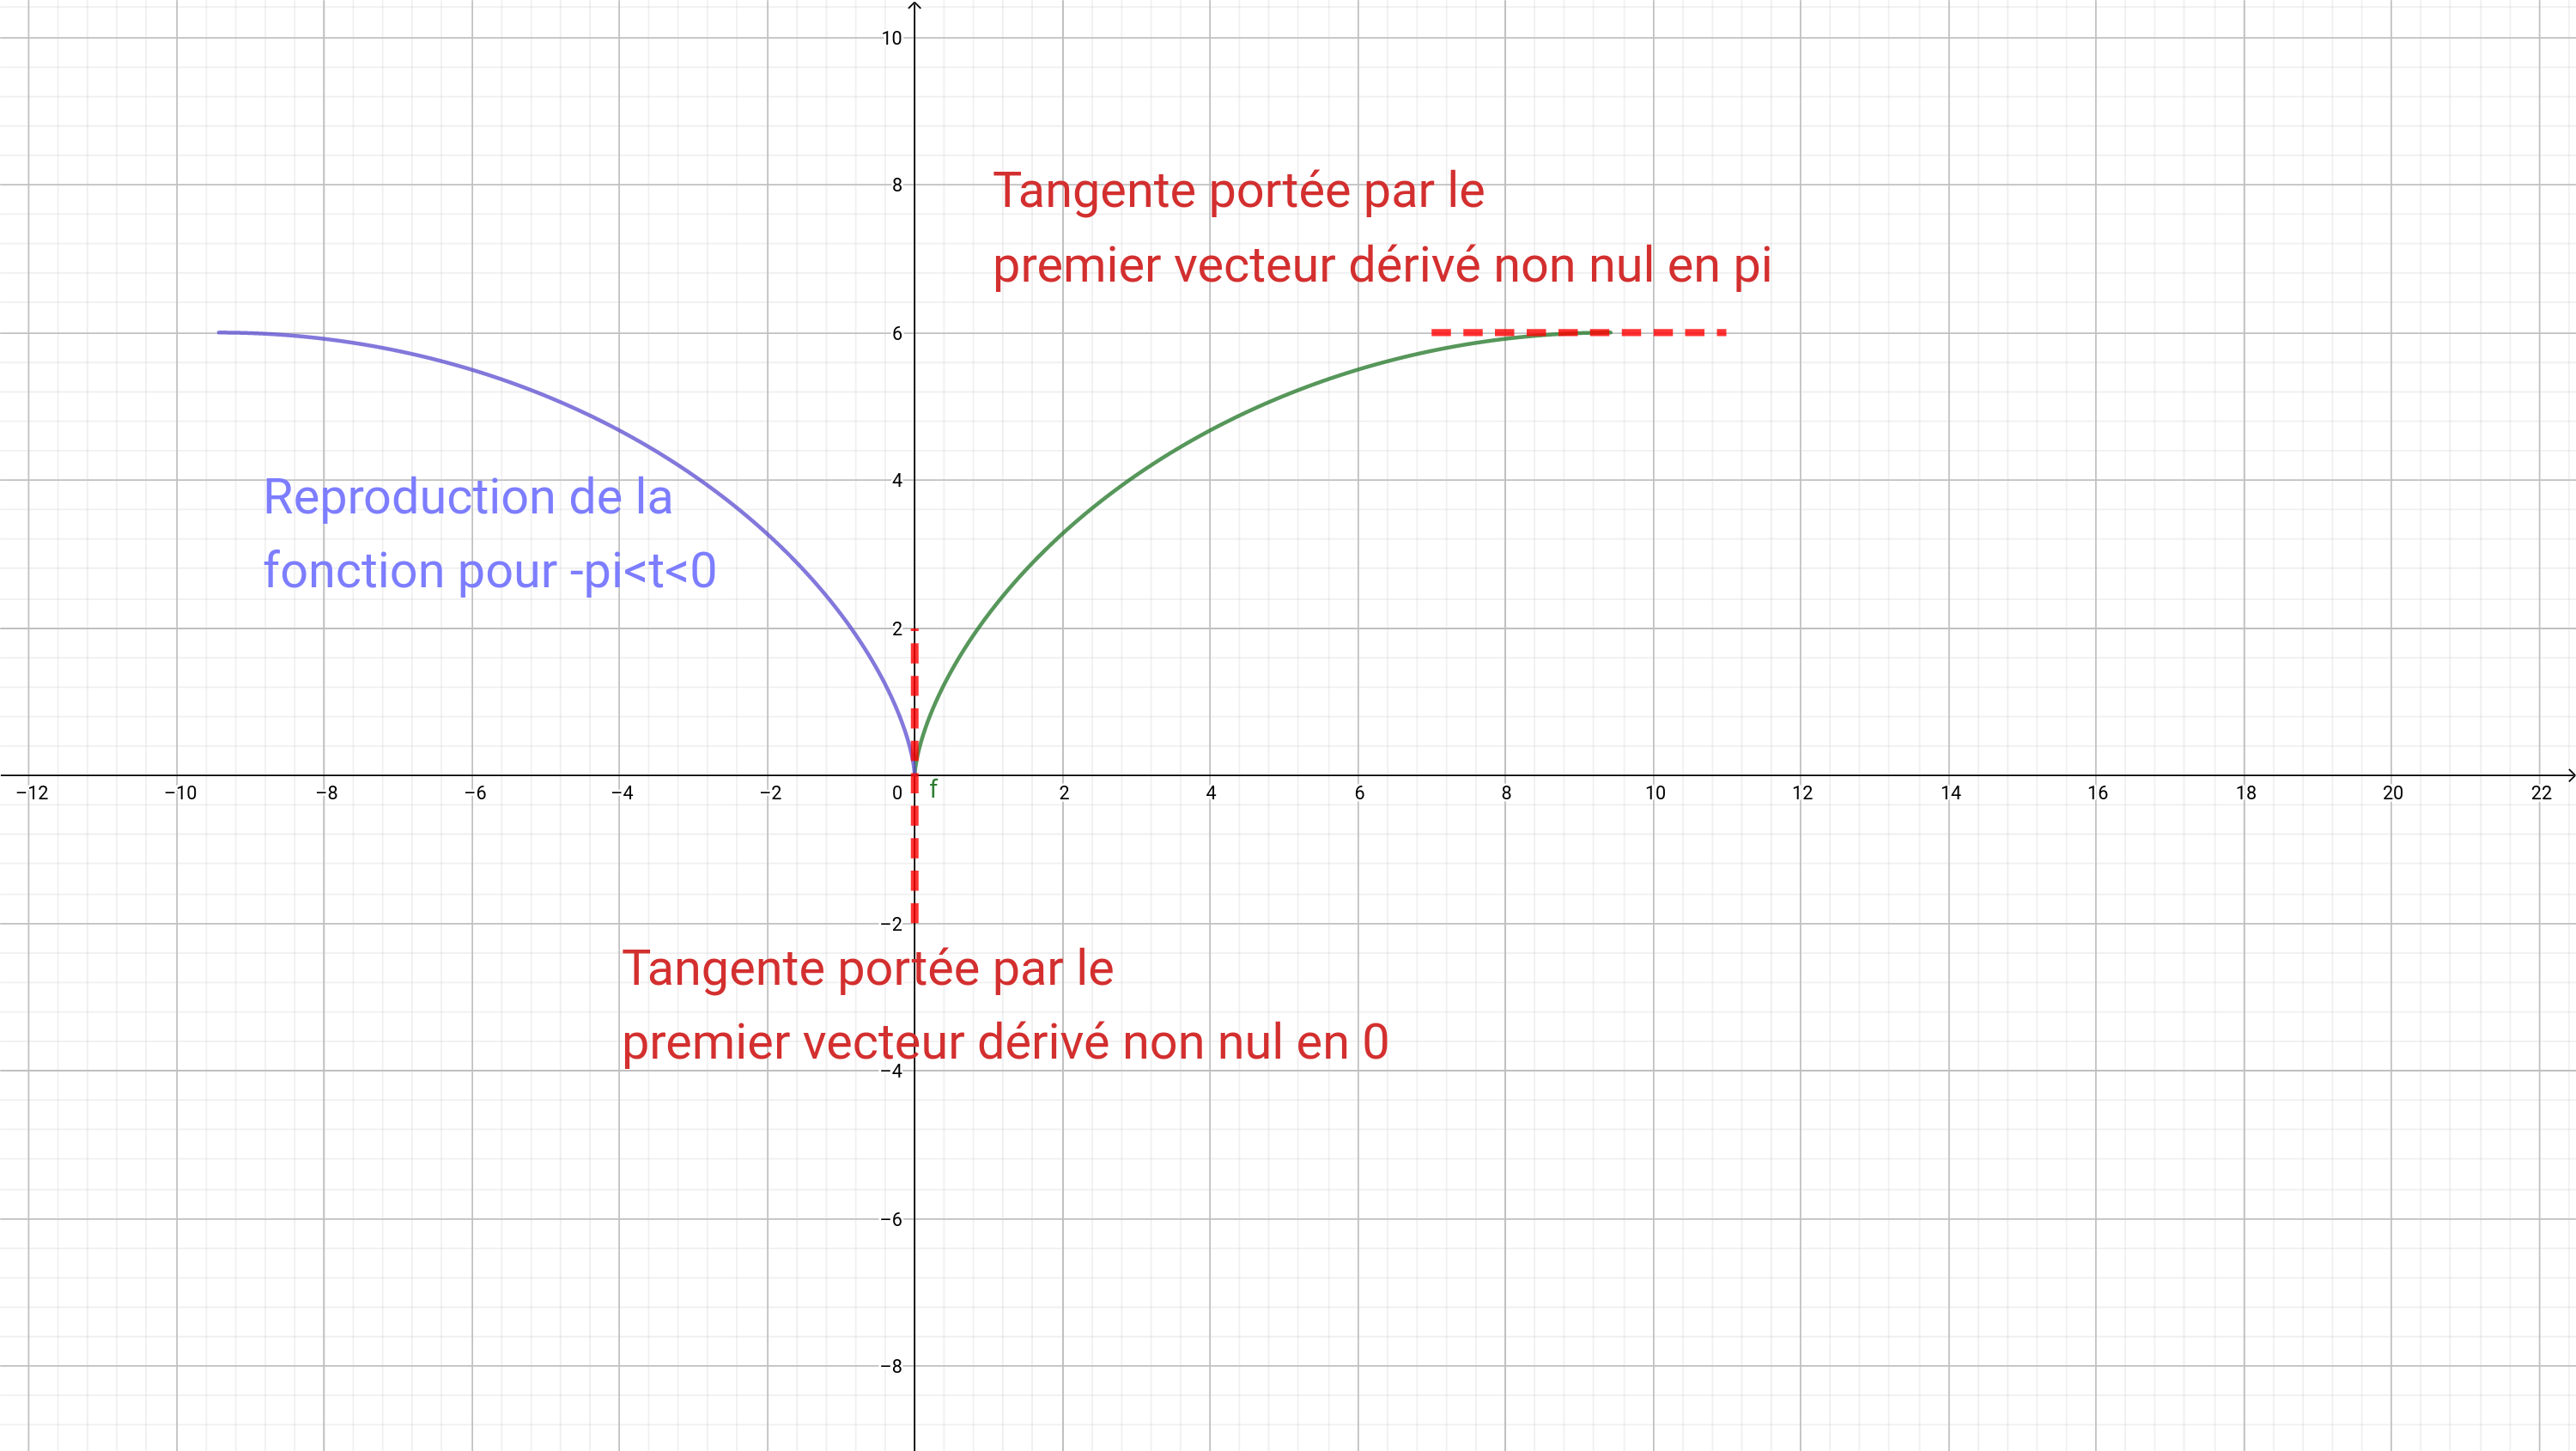
\includegraphics[width=\textwidth]{images/td4ex1q1.png}
\begin{tikzpicture}[scale=.75]
        \draw [very thin, gray!10] (-10,-1) grid[step=0.2] (12,7);
        \draw [very thin, gray!25] (-10,-1) grid[step=1.0] (12,7);
        \foreach \y in { 0,2,...,6} \draw(0,\y)node[left]{\y};
        \foreach \x in {-8,-6,...,9} \draw(\x,0)node[below]{\x};
        \draw[->] (-9.5,0) -- (9.5,0) node[right] {$x$};
        \draw[->] (0,-1) -- (0,6.5) node[above] {$y$};
        \draw[green, thick] [domain=  0:pi] plot ({3*(\x - sin(\x r))}, {3*(1 - cos(\x r))});
        \draw[blue,thick] [domain=-pi:0 ] plot ({3*(\x - sin(\x r))}, {3*(1 - cos(\x r))});
        \draw[<->,red, very thick] (0,-0.5) -- (0,0.5);
        \draw[<->,red, very thick] ({3*pi+0.5},{6}) -- ({3*pi-0.5},{6});
        \draw[red] (9,5) node {\parbox{5cm}{Tangente portée par le premier vecteur non nul en $t=\pi$}};
        \draw[red] (4,1) node {\parbox{5cm}{Tangente portée par le premier vecteur non nul en $t=0$}};
        \draw[blue] (-6,3) node {\parbox{5cm}{Reproduction de la courbe pour $t\in[-\pi;0]$}};
\end{tikzpicture}

\solution{}
\section{Obtention de $(C)$ à partir de $(\Gamma)$}
La courbe n'a pas de périodicité comme nous l'avons vu à la question 1.
Cependant, on remarque que $x(t)$ et $y(t)$ contiennent des fonctions trigonométriques qui sont
$2\pi$ périodiques.
En regardant plus attentivement, on voit que $x(t)$ n'est pas périodique car elle contient
$t$.
Mais $y(t)$ est périodique, en effet, on peut écrire~:
\begin{align*}
        y(t) = 3[1-\cos t] = 3 - 3\cos t
\end{align*}
Donc $y(t)$ a la même période que $\cos t$, c'est-à-dire $2\pi$.
On peut le vérifier~:
\begin{align*}
        y(t+2\pi) &= 3-\cos (t+2\pi)\\
                  &= 3-\cos(t)\\
                  &= y(t)
\end{align*}
La fonction $y(t)$ est $2\pi$ périodique signifie que tous les $2\pi$, la fonction $y(t)$
reprend les mêmes valeurs et ceci sur tout l'ensemble de définition.
Quel est le comportement de $x(t)$ tous les $2\pi$?
Pour répondre à cette question, on calcule~:
\begin{align*}
        x(t+2\pi) &= 3[t+2\pi-\sin(t+2\pi)]\\
                  &= 6\pi+3[t-\cos t]\\
                  &= 6\pi+x(t)
\end{align*}
Que peut-on conclure de ceci?
On considère un point $M(t)$ et le point $M(t+2\pi)$ le vecteur translation entre
ces points peut être calculé comme $\vec{u}=M(t+2\pi)-M(t)$~:
\begin{align*}
        \vec{u}&=\left|\begin{array}{l}x(t+2\pi)-x(t)\\y(t+2\pi)-y(t)\end{array}\right.\\
        \vec{u}&=\left|\begin{array}{l}6\pi\\0\end{array}\right.
\end{align*}
On peut donc obtenir la courbe $(C)$ à partir de $(\Gamma)$ en faisant des transations
de vecteur $\vec{u}$~:\\
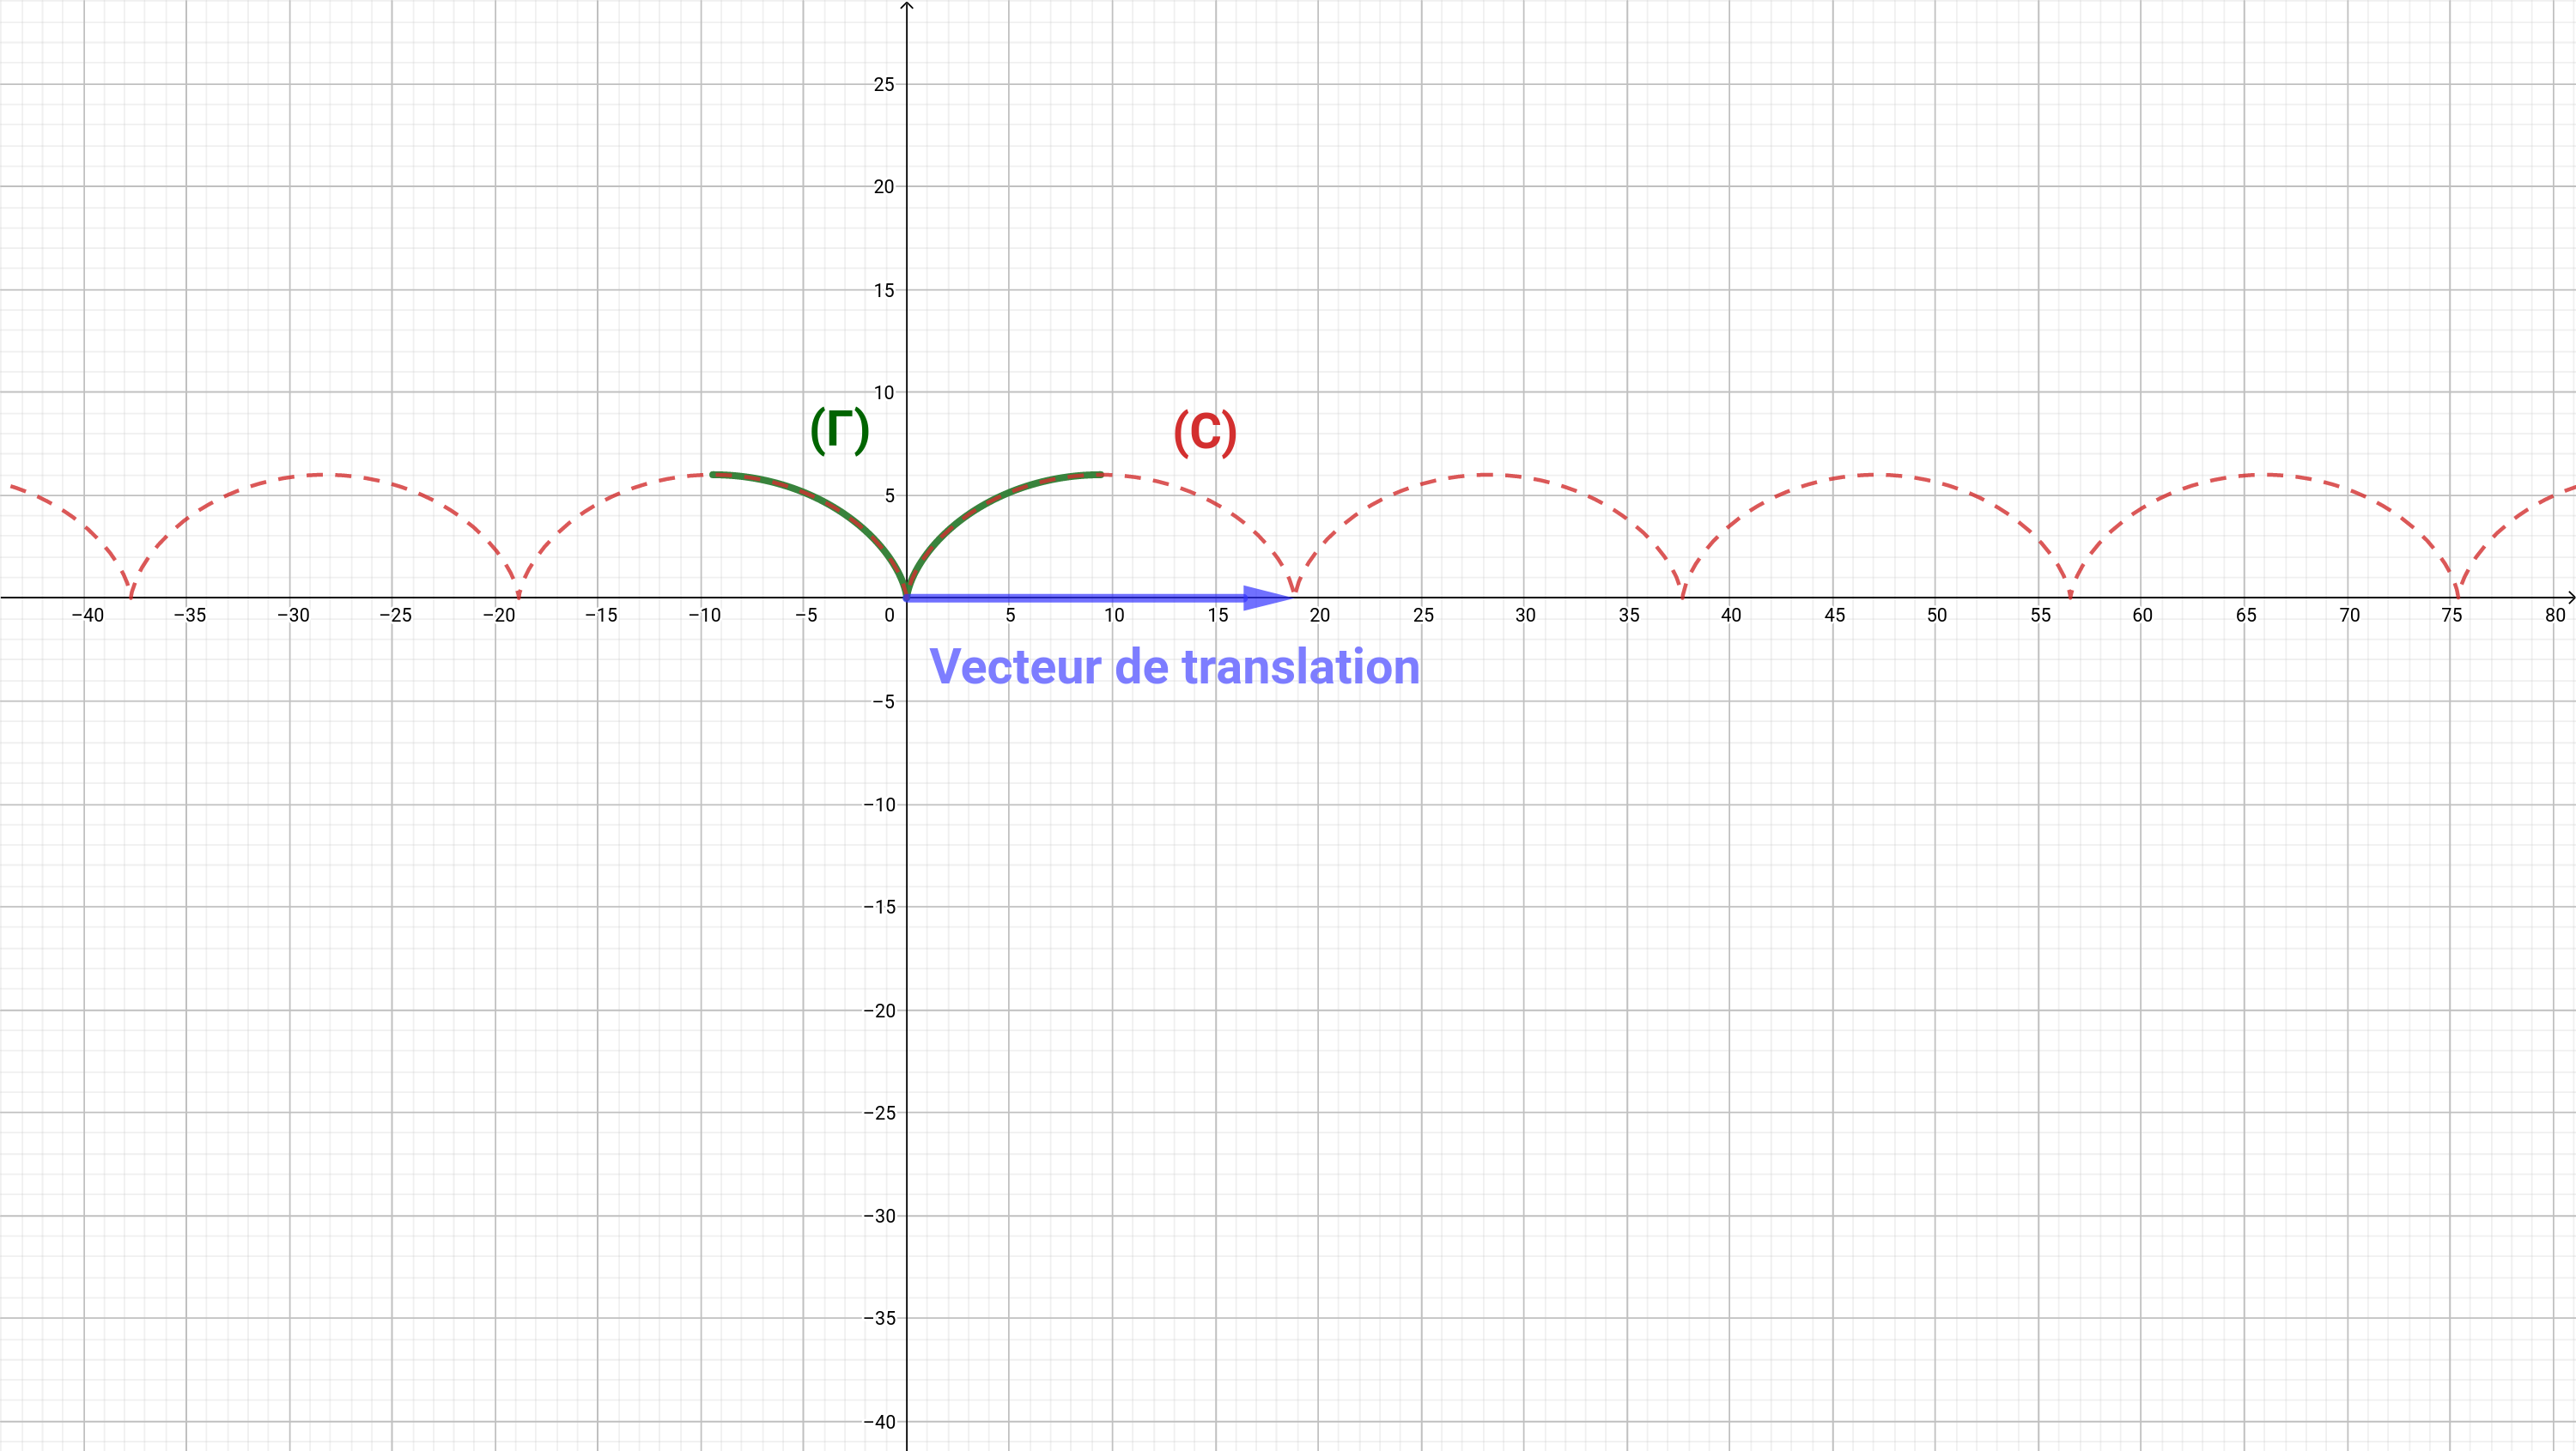
\includegraphics[width=\textwidth]{images/td4ex1q2.png}
Cette courbe est la cycloïde.
C'est le lieu géométrique d'un point fixé sur un cercle qui roule
sans glisser sur une droite.\footnote{\url{https://fr.wikipedia.org/wiki/Cycloïde}}

\exo{}
Étudier la courbe définie par la représentation~:
\begin{align*}
\left\{%
\begin{array}{l}
x(t) = \cos^3 t\\
y(t) = \sin^3 t
\end{array}%
\right.
\end{align*}
\solution{}
\section{Domaines de définition et d'étude}
\subsection{Domaine de définition}
L'ensemble de définition est l'intersection de l'ensemble de définition de $x()$ et de $y(t)$:
\begin{align*}
        D&=D_x\cap D_y\\
         &=\mathbb{R}\cap \mathbb{R}\\
         &=\mathbb{R}
\end{align*}
\subsection{Domaine d'étude}
\subsubsection{Périodicité}
Les fonctions $\cos$ et $\sin$ sont $2\pi$ périodiques.
On étudiera la courbe sur un intervalle d'amplitude $2\pi$.
Comme l'on souhaite utiliser la parité, on choisira comme intervalle d'étude
un intervalle symétrique par rapport à l'origine.
On choisit donc $[-\pi;\pi]$.
\subsubsection{Parité}
\begin{align*}
\left\{%
\begin{array}{l}
        x(-t) = (\cos(-t))^3 =  \cos^3 t = x(t)\\
        y(-t) = (\sin(-t))^3 = -\sin^3 t = -y(t)\\
\end{array}%
\right.
\end{align*}
On est dans le cas où l'on étudiera la courbe sur $[0;\pi]$
puis on fera la symétrie par rapport à $(Ox)$. Notre intervalle d'étude sera donc
$[0;\pi]$.
\section{Tableau de variations sur $[0;\pi]$}
\subsection{Variations}
\begin{align*}
        x'(t) &= -3\sin(t)\cos^2(t)\\
        x'(t) &\ge 0 \text{ car } \sin(t)\ge 0 \text{ et } \cos^2(t)\ge 0 \text{ sur } [0;\pi]\\
        \\
        y'(t) &= 3\cos(t)\sin^2(t)\\
        &\text{or } \sin^2(t)\ge 0\\
        &\text{Si } t\in[0;\frac{\pi}{2}]\text{, } \cos t \ge 0 \text{ donc } y'(t)\ge 0\\
        &\text{Si } t\in[\frac{\pi}{2}; \pi]\text{, } \cos t \le 0 \text{ donc } y'(t)\le 0
\end{align*}
\begin{align*}
        x(0) &=\cos^3(0)=1 & x(\frac{\pi}{2})&=\cos^3(\frac{\pi}{2})=0 & x(\pi) &= \cos^3(\pi) = -1\\
        y(0) &=\sin^3(0)=1 & x(\frac{\pi}{2})&=\sin^3(\frac{\pi}{2})=1 & x(\pi) &= \sin^3(\pi) =  0\\
        x'(0)&=-3\sin(0)\cos^2(0)=0 & x'(\frac{\pi}{2})&=-3\sin(\frac{\pi}{2})\cos^2(\frac{\pi}{2})=0 & x'(\pi) &= -3\sin(\pi)\cos^2(\pi) = 0\\
        y'(0)&= 3\cos(0)\sin^2(0)=0 & x'(\frac{\pi}{2})&= 3\cos(\frac{\pi}{2})\sin^2(\frac{\pi}{2})=0 & x'(\pi) &=  3\cos(\pi)\sin^2(\pi) = 0\\
\end{align*}
Donc~:\\
\begin{tikzpicture}
        \tkzTabInit{$t$ / 1 , $x'(t)$ / 1, $x(t)$ / 1, $y'(t)$ / 1, $y(t)$ / 1}{$0$, $\frac{\pi}{2}$, $+\pi$}
        \tkzTabLine{0,-,0,-,0}
        \tkzTabVar{+/ $1$ ,R/, -/ $-1$}
        \tkzTabIma{1}{3}{2}{$0$}
        \tkzTabLine{0,+,0,-,0}
        \tkzTabVar{-/ $0$ , +/ $1$, -/ $0$}
\end{tikzpicture}
\subsection{Tangentes}
On détermine les tangentes en $0$, en $\frac{\pi}{2}$ et en $\pi$.
On cherche donc en ces points le premier vecteur dérivé non nul.\\
On appelle $A$ le point de la courbe en $t=0$.
\begin{align*}
        A&=\left|\begin{array}{l}x(0)\\y(0)\end{array}\right.\\
                A&=\left|\begin{array}{l}1\\0\end{array}\right.
\end{align*}
En $A$~:
\begin{align*}
        \vec{F}'(0)&=\left|\begin{array}{l}
                x'(0)\\y'(0)
        \end{array}\right.
        =          \left|\begin{array}{l}
                0\\0
        \end{array}\right.\\
        \vec{F}"(t)&=\left|\begin{array}{l}
                -3[\cos(t)\cos^2(t) - \sin(t)\times 2\sin(t)\cos(t)]\\
                 3[\sin(t)\sin^2(t) - \cos(t)\times 2\cos(t)\sin(t)]\\
        \end{array}\right.\\
        \vec{F}"(0)&=\left|\begin{array}{l}
                -3\\0
        \end{array}\right.
\end{align*}
$\vec{F}"(0)$ est donc le premier vecteur dérivé non nul en $t=0$, il dirigera donc la tangente en $A(1;0)$.\\
On appelle $B$ le point de la courbe en $t=\frac{\pi}{2}$.
\begin{align*}
        B&=\left|\begin{array}{l}x(\frac{\pi}{2})\\y(\frac{\pi}{2})\end{array}\right.\\
                B&=\left|\begin{array}{l}0\\1\end{array}\right.
\end{align*}
En $B$~:
\begin{align*}
        \vec{F}'(\frac{\pi}{2})&=\left|\begin{array}{l}
                x'(\frac{\pi}{2})\\y'(\frac{\pi}{2})
        \end{array}\right.
        =          \left|\begin{array}{l}
                0\\0
        \end{array}\right.\\
        \vec{F}"(\frac{\pi}{2})&=\left|\begin{array}{l}
                 0\\-3
        \end{array}\right.
\end{align*}
$\vec{F}"(\frac{\pi}{2})$ est donc le premier vecteur dérivé non nul en $t=\frac{\pi}{2}$, il dirigera donc la tangente en $B(0;1)$.\\
On appelle $C$ le point de la courbe en $t=\pi$.
\begin{align*}
        C&=\left|\begin{array}{l}x(\pi)\\y(\pi)\end{array}\right.\\
                C&=\left|\begin{array}{l}-1\\0\end{array}\right.
\end{align*}
En $C$~:
\begin{align*}
        \vec{F}'(\pi)&=\left|\begin{array}{l}
                x'(\pi)\\y'(\pi)
        \end{array}\right.
        =          \left|\begin{array}{l}
                0\\0
        \end{array}\right.\\
        \vec{F}"(\pi)&=\left|\begin{array}{l}
                 3\\0
        \end{array}\right.
\end{align*}
$\vec{F}"(\pi)$ est donc le premier vecteur dérivé non nul en $t=\pi$, il dirigera donc la tangente en $C(-1;0)$.\\
\section{Branches infinies}
Il n'y a ni borne infinie, ni valeur interdite, donc pas de branche infinie à étudier.
\section{Tracé de la courbe}
Voir le tracé pas à pas sur ametice.

Cette courbe est appelée astroïde.
Elle représente le lieu géométrique d'un point d'un cercle qui roule sans glisser
à l'intérieur d'un cercle de rayon supérieur.\footnote{\url{https://fr.wikipedia.org/wiki/Astroïde}}

\exo{}
Étudier la courbe définie par la représentation~:
\begin{align*}
\left\{%
\begin{array}{l}
        x(t) = \frac{1}{t}+\ln(2+t)\\
        y(t) = t+\frac{1}{t}
\end{array}%
\right.
\end{align*}
\solution{}
\section{Domaines de définition et d'étude}
\subsection{Domaine de définition}
À cause du $\frac{1}{t}$, on a $t\ne 0$.
À cause du $\ln$, on a $t>-2$.
On en déduit que~:
\begin{align*}
        D=\left]-2;0\right[\cup\left]0;\infty\right[
\end{align*}
\subsection{Domaine d'étude}
Les fonctions utilisées n'ont ni période, ni parité, donc~:
\begin{align*}
        I=\left]-2;0\right[\cup\left]0;\infty\right[
\end{align*}
\section{Tableau de variations sur $I$}
\begin{align*}
        x\;'(t) & = -\frac{1}{t^2}+\frac{1}{2+t}\\
                & = -\frac{-2-t+t^2}{t^2(2+t)}
\end{align*}
Le dénominateur est positif car $t^2>0$ et $2+t>0$ car $t\in\left]-2;0\right[\cup\left]0;\infty\right[$.
donc $x\;'(t)$ a le signe de $t^2-t-2$.
$t^2-t-2$ a pour racine $2$ et $-1$ (on peut calculer ces racines grâce au $\Delta$ (ici $\Delta=9$) ou
en cherchant des racines évidentes).
Le tableau de signe de $t^2-t-2$ est~:\\
\begin{tikzpicture}
        \tkzTabInit{$t$ / 1 , signe de $t^2-t-2$ / 1}{$-\infty$, $-1$, $2$, $+\infty$}
        \tkzTabLine{,+,0,-,0,+,}
\end{tikzpicture}

\begin{align*}
        y\;'(t) &= 1-\frac{1}{t^2} \\
                &= \frac{t^2-1}{t^2}
\end{align*}
$y\;'(t)$ a le signe de $t^2-1$.\\
\begin{tikzpicture}
        \tkzTabInit{$t$ / 1 , signe de $t^2-1$ / 1}{$-\infty$, $-1$, $+1$, $+\infty$}
        \tkzTabLine{,+,0,-,0,+,}
\end{tikzpicture}
\begin{align*}
        \lim_{t\to -2} x(t)              & = -\infty &
        \lim_{\substack{t\to 0\\<}} x(t) & = -\infty &
        \lim_{\substack{t\to 0\\>}} x(t) & = +\infty &
        \lim_{{t\to +\infty}}       x(t) & = +\infty \\
        x(-1)                            & = -1      &
        x(1)                             & = 1+\ln 3 &
        x(2)                             & = \frac{1}{2} + \ln 4 &
        x\;'(1)                          & = -\frac{2}{3} \\
        \lim_{t\to -2} y(t)              & = -\frac{5}{2} &
        \lim_{\substack{t\to 0\\<}} y(t) & = -\infty &
        \lim_{\substack{t\to 0\\>}} y(t) & = +\infty &
        \lim_{{t\to +\infty}}       y(t) & = +\infty \\
        y(-1)                            & = -2      &
        y(1)                             & = 2       &
        y(2)                             & = \frac{5}{2} &
        y\;'(2)                          & = \frac{3}{4} \\
\end{align*}
D'où le tableau de variations~:\\
\begin{tikzpicture}
        \tkzTabInit{$t$ / 1 , $x\;'(t)$ / 1, $x(t)$ / 2, $y\;'(t)$ / 1, $y(t)$ / 2}{$-2$, $-1$, $0$, $+1$, $+2$, $+\infty$}
        \tkzTabLine{d , + , 0 , - , d , - , -\frac{2}{3}, -, 0, +, }
        \tkzTabVar{-D- / / $-\infty$ , +/ -1, -D+ / $-\infty$ / $+\infty$, R/, -/ $\frac{1}{2}+\ln 4$, +/ $+\infty$}
        \tkzTabIma{3}{5}{4}{$1+\ln 3$}
        \tkzTabLine{d , + , 0 , - , d , - , 0, +, \frac{3}{4} , +, }
        \tkzTabVar{-D- / / $-\frac{5}{2}$ , +/ -2, -D+ / $-\infty$ / $+\infty$, -/ 2, R/, +/ $+\infty$}
        \tkzTabIma{4}{6}{5}{$\frac{5}{2}$}
\end{tikzpicture}
\section{Tangentes}
Pour $t=-1$, on a le point $A\left|\begin{array}{c}-1\\-2\end{array}\right.$.
        Or $F\;'(-1) = \left|\begin{array}{c}0\\0\end{array}\right.$ et
                $F\;"(-1) = \left|\begin{array}{c}-3\\-2\end{array}\right.$.
                        $F\;"(-1)$ est donc le premier vecteur dérivé non nul en $-1$, il dirige
                        donc la tangente en $A$.\\
Pour $t=1$, on a le point $B\left|\begin{array}{c}1+\ln 3\\2\end{array}\right.$.
        $F\;'(1) = \left|\begin{array}{c}-\frac{2}{3}\\0\end{array}\right.$
                        $F\;'(1)$ est donc le premier vecteur dérivé non nul en $1$, il dirige
                        donc la tangente en $B$.\\
Pour $t=2$, on a le point $C\left|\begin{array}{c}\frac{1}{2}+\ln 4\\\frac{5}{2}\end{array}\right.$.
        $F\;'(2) = \left|\begin{array}{c}0\\\frac{3}{4}\end{array}\right.$
                $F\;'(2)$ est donc le premier vecteur dérivé non nul en $2$, il dirige
                        donc la tangente en $C$.\\
\section{Branches infinies}
\begin{itemize}
\item Pour $t=-2$, on a~:
\begin{align*}
        \lim_{t\to -2} x(t)              & = -\infty &
        \lim_{t\to -2} y(t)              & = -\frac{5}{2}
\end{align*}
Donc la droite $y=-\frac{5}{2}$ est asymptote à la courbe au voisinage de $t=-2$.
\item Pour $t=0$, on a~:
\begin{align*}
        \lim_{\substack{t\to 0\\<}} x(t) & = -\infty &
        \lim_{\substack{t\to 0\\>}} x(t) & = +\infty \\
        \lim_{\substack{t\to 0\\<}} y(t) & = -\infty &
        \lim_{\substack{t\to 0\\>}} y(t) & = +\infty
\end{align*}
                On doit donc étudier $\lim_{t\to 0}\frac{y(t)}{x(t)}$.
\begin{align*}
        \frac{y(t)}{x(t)} &= \frac{t+\frac{1}{t}}{\frac{1}{t}+\ln(2+t)}\\
                          &= \frac{\frac{t^2+1}{t}}{\frac{1+t\ln(2+t)}{t}} \\
                          &= \frac{t^2+1}{1+t\ln(2+t)}
\end{align*}
Donc $\lim_{t\to 0}\frac{y(t)}{x(t)}=1$.
                Comme $\lim_{t\to 0}\frac{y(t)}{x(t)}=1$, on doit étudier
                $\lim_{t\to 0}[y(t)-1\times x(t)]$ (Cas n$^o$3 du cours).
\begin{align*}
        y(t)-x(t) & = (t+\frac{1}{t})-(\frac{1}{t}+\ln(2+t))\\
                  & = t-\ln(2+t)
\end{align*}
                Donc $\lim_{t\to 0}[y(t)-1\times x(t)]=-\ln 2$.
                On en déduit que $y=x-\ln 2$ est asymptote au voisinage de $t=0$.
\item Pour $t=+\infty$, on a~:
\begin{align*}
        \lim_{{t\to +\infty}}       x(t) & = +\infty &
        \lim_{{t\to +\infty}}       y(t) & = +\infty 
\end{align*}
On doit étudier $\lim_{t\to +\infty}\frac{y(t)}{x(t)}$.
On factorise le numérateur et le dénominateur par leur terme le plus fort en $t$:
\begin{align*}
        \frac{y(t)}{x(t)} &= \frac{t^2(1+\frac{1}{t^2}}{t\ln(2+t)\left[\frac{1}{t\ln(2+t)}+1\right]} \\
                          &= \frac{t}{\ln(2+t)}\left[\frac{1+\frac{1}{t^2}}{\frac{1}{t\ln(2+t)}+1}\right]
\end{align*}
On voit que le terme entre crochets tend vers 1 lorsque $t\to +\infty$.
Pour le premier terme, il faut faire apparaître au numérateur et au dénominateur
                le même terme en $t+2$ pour utiliser le théorème des croissances composées.\\
                \textbf{Rappel:} théorème des croissances composées~:\\
\begin{align*}
        \lim_{t\to +\infty}\frac{t^\alpha}{\left(\ln t\right)^\beta}&=+\infty & \alpha>0\;\beta>0 & &  & & & & 
\end{align*}
Donc on réécrit la limite de la façon suivante~:
\begin{align*}
        \frac{y(t)}{x(t)} &= \left(\frac{t+2}{\ln(2+t)}\right)
                             \left(\frac{t}{t+2}\right)
                             \left[\frac{1+\frac{1}{t^2}}{\frac{1}{t\ln(2+t)}+1}\right]
\end{align*}
Le premier terme tend vers $+\infty$ selon le théorème des croissances composées, le second
tend vers $1$ et le troisième vers $1$.
On en déduit que la limite tend vers $+\infty$.
                Donc, la courbe admet au voisinage de $t=+\infty$ une branche parabolique d'axe $(Oy)$.
\end{itemize}

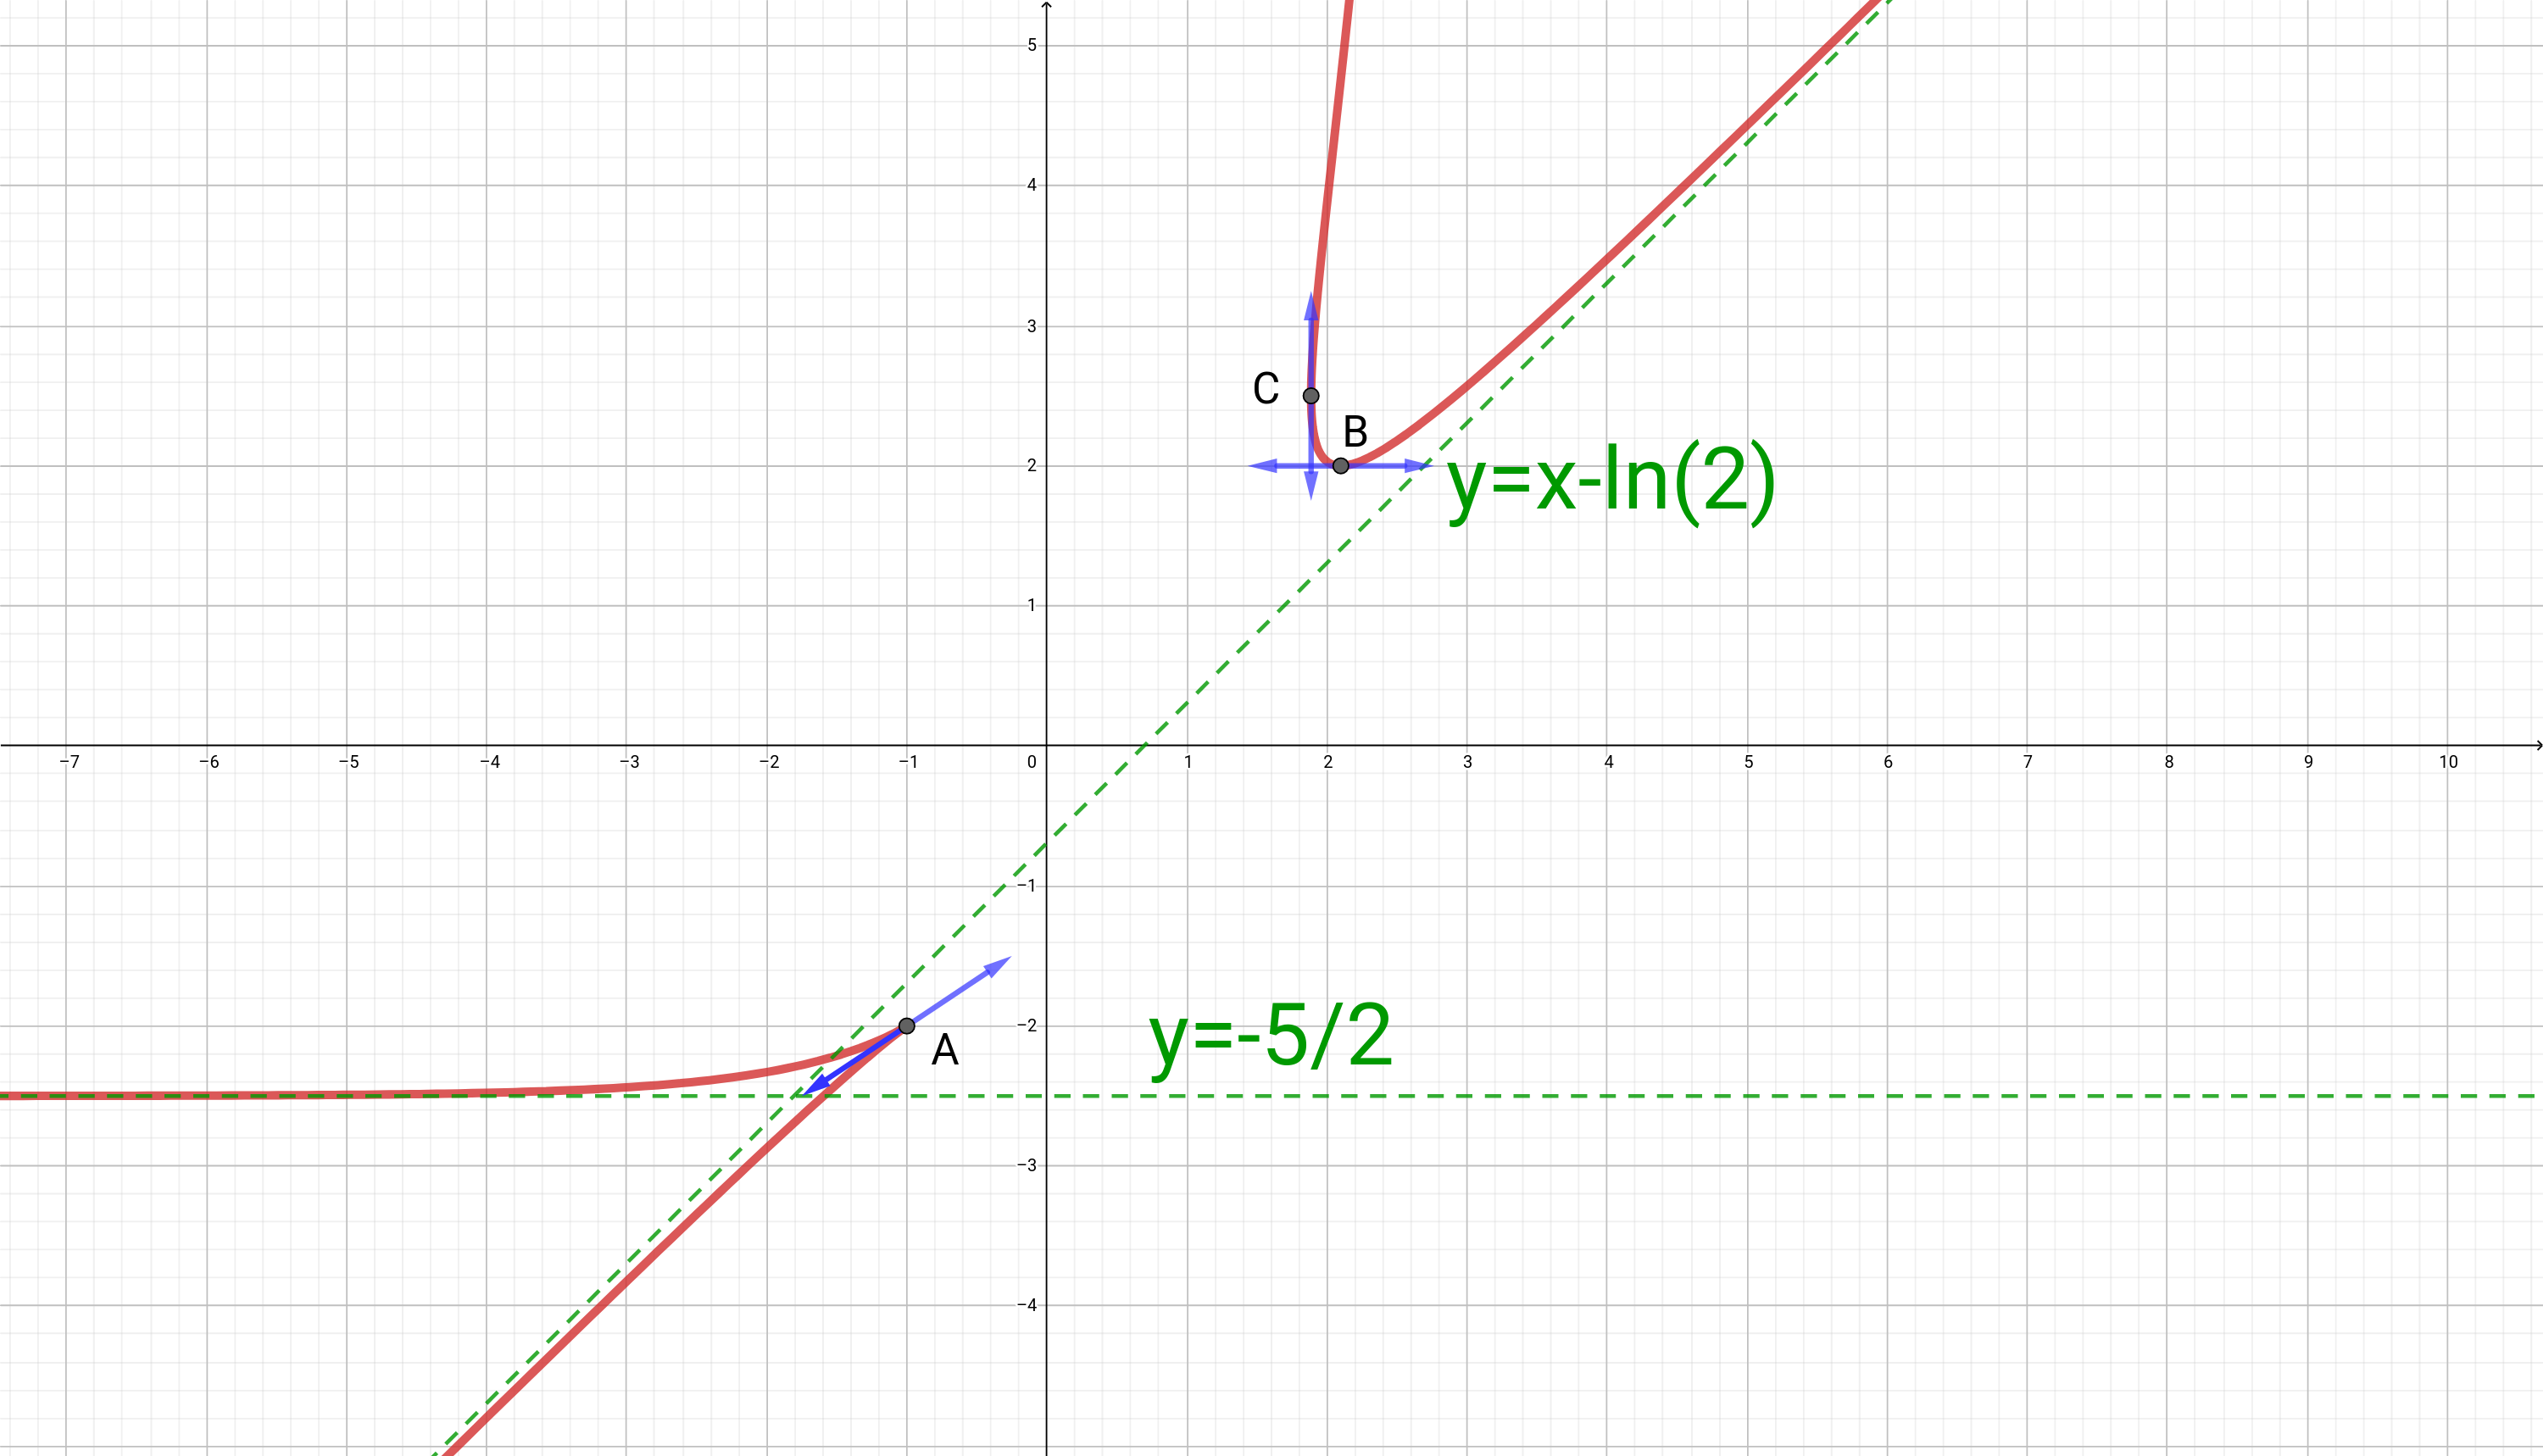
\includegraphics[width=\textwidth]{images/exercice3.png}
\end{document}
